\documentclass[11pt, letterpaper]{article}
\usepackage[margin=0.5in]{geometry}
\usepackage{graphicx}

\begin{document}

\title{Assingment 1: Genetic Drift}
\author{Ryan Layer}
\maketitle

\section{Introduction}
Genetic drift is a mechanism of evolution that influences allele frequencies in
populations. It occurs due to random sampling of alleles during the formation
of gametes, leading to changes in allele frequencies in the subsequent
generation. Unlike natural selection, genetic drift does not act on the basis
of the fitness of alleles; instead, it operates purely by chance.

\section{Results}
In a random mating simulation(Figure~ref{fig:drift} with no selection, five
samples, ten loci where, and the number of offspring was uniformly distributed
between zero and five, one allele was lost, and another reached fixation. {\bf In
this simulation, on average, an allele was lost 52.2\% of the time, and an
allele reached fixation 60.3\% of the time.}

\begin{figure}[h]
    \centering
    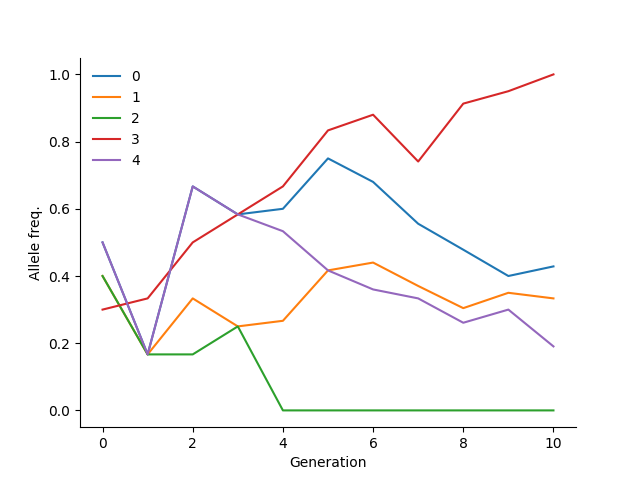
\includegraphics[width=0.5\textwidth]{fig1}
    \caption{The allele frequency of each generation of A random mating
    simulation with five samples, ten loci, and at most five offspring.}
    \label{fig:drift}
\end{figure}

\section{Methods}


Samples were represented by lists of alleles, where each was either a one or
zero, corresponding to the sample having or not having that allele. At each
generation, samples were randomly paired and the number of their offspring was
randomly selected. For each offspring, alleles were determined by randomly
selecting a parently value. Once all offspring alleles were set, the parents
were removed from the simulation. At each round, the allele frequency of each
allele was determined by inspecting all of the offspring.

Figure~\ref{fig:drift} visualizes the allele frequency at each generation for
one simulation.  {\bf To get the fixation and loss statics, the simulation was run
1,000 times, and the final allele frequency was tested for either a zero (loss)
or a one (fixation).}

To run the software, first clone the repository, then run the allele frequency
simulation as follows:
\begin{verbatim}
$ clone 
$ python af.py --num_samples 10 --num_sites 10 --max_offspring 5
\end{verbatim}

\end{document}
